\documentclass[11pt,a4paper]{report}
\usepackage[utf8]{inputenc}
\usepackage{amsmath}
\usepackage{amsthm}
\usepackage{color}
\usepackage[a4paper]{geometry}
\usepackage{listings}
\usepackage{xcolor}
\usepackage{dirtytalk}
\UseRawInputEncoding
\usepackage{graphicx}
\usepackage{caption}
\usepackage{subcaption}
\usepackage{mathtools}
\usepackage[thinc]{esdiff}
\usepackage{tocbibind}
\usepackage{parskip}
\newtheorem{theorem}{Theorem}
\newtheorem{definition}{Definition}
\graphicspath{ {./images/} }

\title{Decision Trees and Methods to Optimize Performance}
\author{Pattanin (Mill) Luangamornlert}
\date{\today}

\begin{document}
\maketitle

\begin{abstract}
    \emph{This piece of work is a result of my own work except where it forms an assessment based on group project work. In the case of a group project, the work has been prepared in collaboration with other members of the group. Material from the work of others not involved in the project has been acknowledged and quotations and paraphrases suitably indicated.}
    \bigskip
    
    This project aims to look at methods of Machine Learning, which has been described as the 4th Industrial Revolution (4IR) by the World Economic Forum at Davos in 2016 \cite{Schwab}.
    
    We will look at the mathematics behind Decision Trees, famously described in Leo Breiman's landmark book Classification and Regression Trees \cite{BreimanDT} which is one of the most cited sources for Statistical Machine Learning, with over 48,000 citations.
    
    Breiman, Friedman, Olshen, and Stone noted that CART had its flaws in the book itself and have always strived to improve the method, Breiman introducing Random Forests a few years later, and Friedman created Gradient Boosted Machines in 1999. Since then, many mathematicians have tried to improve upon the work and this project will try to explore these methods.
    \bigskip\\
    \textbf{Key Words:} Classification, Regression, Decision Trees, Metrics, Bootstrap,
    
    
    
\end{abstract}

\tableofcontents

\chapter{An Introduction to Machine Learning}
Machine Learning is a subset of Artificial Intelligence (AI) where we create a mathematical model which can be "trained" using previously known data to create a more robust AI programme which can be deployed in the real world.
We achieve this by using Statistics to create models which we then feed into the machine for it to predict outcomes based on prior events.


\section{Supervised and Unsupervised Learning}
In statistics, there are two objectives which become possible when you look at a data set.

\begin{itemize}
  \item \textbf{Supervised Learning} where we observe how $X$ affects $Y$ as we change the variable $X$
  
  \item \textbf{Unsupervised Learning} we investigate the characteristics of $X$ and how it behaves relative to the rest of the data
\end{itemize}
The methods we will explore will be a Supervised Learning method.\\
There are two main ways to deal with data under Supervised Learning:
\begin{itemize}
    \item \textbf{Classification} - classification is suited when you want to group data together to make predictions which are quantitative. 
    Methods include: Logistic Regression, Support Vector Machines etc.
    
    \item \textbf{Regression} - Regression is the main form of statistical analysis for continuous forms of data as they can be used to build a trend line to estimate an output $Y$ from $X$ based on previously known information.
    Methods include: Linear Regression
\end{itemize}
To see how these work, please consult the following books.
\textbf{An Introduction to Statistical Learning} \cite[Chapter 3-4]{ISLR} 
and \textbf{Elements of Statistical Learning} \cite[Chapter 3-4]{ESL}


\section{What are Decision Trees?}
\textbf{Decision Trees} are essentially a flow chart that is shaped like a tree which is used to make predictions. 
They are a form of non-parametric statistics and a common and easy to interpret alternative for when data is non-linear.
The aim is to input multiple variables (often historical data) into the model, and under supervised learning, we are able to predict the outcome of a future test using the same variables as in the test data.\\
Each decision point is called a "Parent" node, where at each node, we split the set of data into root nodes - called "Child" nodes.
This is done recursively until a stopping point has been achieved.\\
Decision Trees are used widely in industry, such as in medicine where a tree is often used to predict if a patient has cancer or not. 
\medskip\\
Decision Trees provide many advantages over other methods:
\begin{itemize}
    \item They are very easy to understand
    
    \item They do not require lots of effort with regards to data processing
    
    \item Data can be left as is - no normalization or scaling is needed
    
    \item Missing data can be ignored as they do not affect the learning of the model
\end{itemize}

\subsection{Basic History of Decision Trees \cite{50years}} 
The idea of Decision Trees first came out of Operations Research as an optimization problem. This was first developed in 1963 \cite{AID} and the method is called Automatic Interaction Detection (AID).
AID splits the model into subsets and does that recursively until a stopping criteria is met.\\
However, AID is a regression tree algorithm and so development for a classification naturally followed.\\
This ended up being developed into Theta Automatic Interaction Detection (THAID) \cite{THAID}.
THAID splits data using classification methods but had its flaws and was superseded by Chi-square Automatic Interaction Detection (CHAID) \cite{CHAID}. 
In this case we split data into intervals and merge the groups which are not as significant together. From here, Bonferroni corrections are used.\\
Unfortunately, this realistically was not optimal and thus a more optimal method was needed.

\subsection{The CART method - and where do we go on from it?}
Multiple algorithms can be used to create a Decision Tree. 
The most famous of these, Classification and Regression Trees (CART) \cite{BreimanDT} was the first developed by Leo Breiman, Jerome Friedman and others in the 1984 book, Classification and Regression Trees.
Firstly, we will look at how the CART algorithm actually works and show some examples for both classification and regression problems. 
From here we are able to look at the multitude of methods which have been used to improve upon the CART method, such as Random Forest, Gradient Boosting and Optimal Decision Trees.


\section{Programming Language}
For this project, we will be mainly using R as the main programming language although occasionally we might encounter situations where other languages such as Python or Julia turn out to be more convenient/easier to use. This is entirely dependant on the person and their personal preferences.\\
In many cases, it is possible to use at least 2 different languages for the entire process due to the convenience that each bring for the step needed. Often this occurs when we use one
language for data cleansing and another for the analysis and sometimes a third for producing the plots. There is no set order to this and you may use any language you wish.
Note that you will have to install external packages which do not come pre-installed with the programme. In such cases, you will have to install the package before running the code.

\subsubsection{R}
In R \cite{R}, this will be through the Comprehensive R Archive Network (CRAN) which maintains all packages that will be required for this project. When you need to install a new package, run the following line \textit{once}, the first time:
\begin{lstlisting}
install.packages("package")
\end{lstlisting}
To work with data sets we will be using the "dplyr" \cite{dplyr} package which is part of the Tidyverse Library and is used for data manipulation. We will also be using "ggplot2" \cite{ggplot} to produce plots as this package produces better plots than the regular plot function.

\section{Dataset}
The Lahman Dataset is the largest publicly available dataset on baseball. It is part of the Baseball Archive set up by Sean Lahman in 1995 and the Baseball Dataset itself first appeared in 1996 and has been updated annually and maintained by a team of support staff \cite{Lahman} \footnote{Sean Lahman, Chris Dalzell, Michael Friendly, Dennis Murphy, Martin Monkman, Vanessa Foot, Justeena Zaki-Azat}. There is a .csv version, an SQL version, and R version (which is available through the CRAN). We will be using the R version to simplify the necessary data preparation.

\subsubsection{Description}
The following is the description of the data which has been sourced from the Lahman reference manual.\cite{Lahman}\\
\say{\textit{This database contains pitching, hitting, and fielding statistics for Major League Baseball from 1871 through 2019. It includes data from the two current leagues (American and National), the four other "major" leagues (American Association, Union Association, Players League, and Federal League), and the National Association of 1871-1875.
This database was created by Sean Lahman, who pioneered the effort to make baseball statistics freely available to the general public. What started as a one man effort in 1994 has grown tremendously, and now a team of researchers have collected their efforts to make this the largest and most accurate source for baseball statistics available anywhere.}}\footnote{CRAN reference manual: https://cran.r-project.org/web/packages/Lahman/Lahman.pdf}

\subsection{Variables in data}
We have selected two sets of data to work on this project, one each for classification and regression. Below is the code for the data and the variables we have selected in each.

\subsubsection{Playoff - Classification}
The following is to predict whether a team would win the league given how well a team did throughout the season. Here is the code to isolate the data:
\subsubsection{Training Data}
\begin{lstlisting}[basicstyle=\scriptsize]
teamseason <- Lahman::Teams
head(teamseason)

alplayoff <- filter(teamseason, teamseason$lgID =="AL")
head(alplayoff)
is.factor(alplayoff)
alplayoff[alplayoff =="N"] = 0
alplayoff[alplayoff =="Y"] = 1
head(alplayoff)
alplayoff %>% filter(!is.na(LgWin))
alplayoff1 = subset(alplayoff, select = -c(Rank, park, WSWin, 
                                           name, teamID, franchID, teamIDBR,
                                           teamIDlahman45, teamIDretro))
alplayoff1$LgWin <- as.factor(alplayoff1$LgWin)
alplayoff1[is.na(alplayoff1)] <- 0

\end{lstlisting}

\subsubsection{Testing Data}
\begin{lstlisting}[basicstyle=\scriptsize]
nlplayoff <- filter(teamseason, teamseason$lgID =="NL")
head(nlplayoff)
is.factor(nlplayoff)
nlplayoff[nlplayoff =="N"] = 0
nlplayoff[nlplayoff =="Y"] = 1
head(nlplayoff)
nlplayoff %>% filter(!is.na(LgWin))
nlplayoff1 = subset(nlplayoff, select = -c(Rank, park, WSWin, 
                                           name, teamID, franchID, teamIDBR,
                                           teamIDlahman45, teamIDretro))
nlplayoff1$LgWin <- as.factor(nlplayoff1$LgWin)
nlplayoff1[is.na(nlplayoff1)] <- 0
\end{lstlisting}



\subsubsection{Salary - Regression}
\begin{figure}
    \centering
    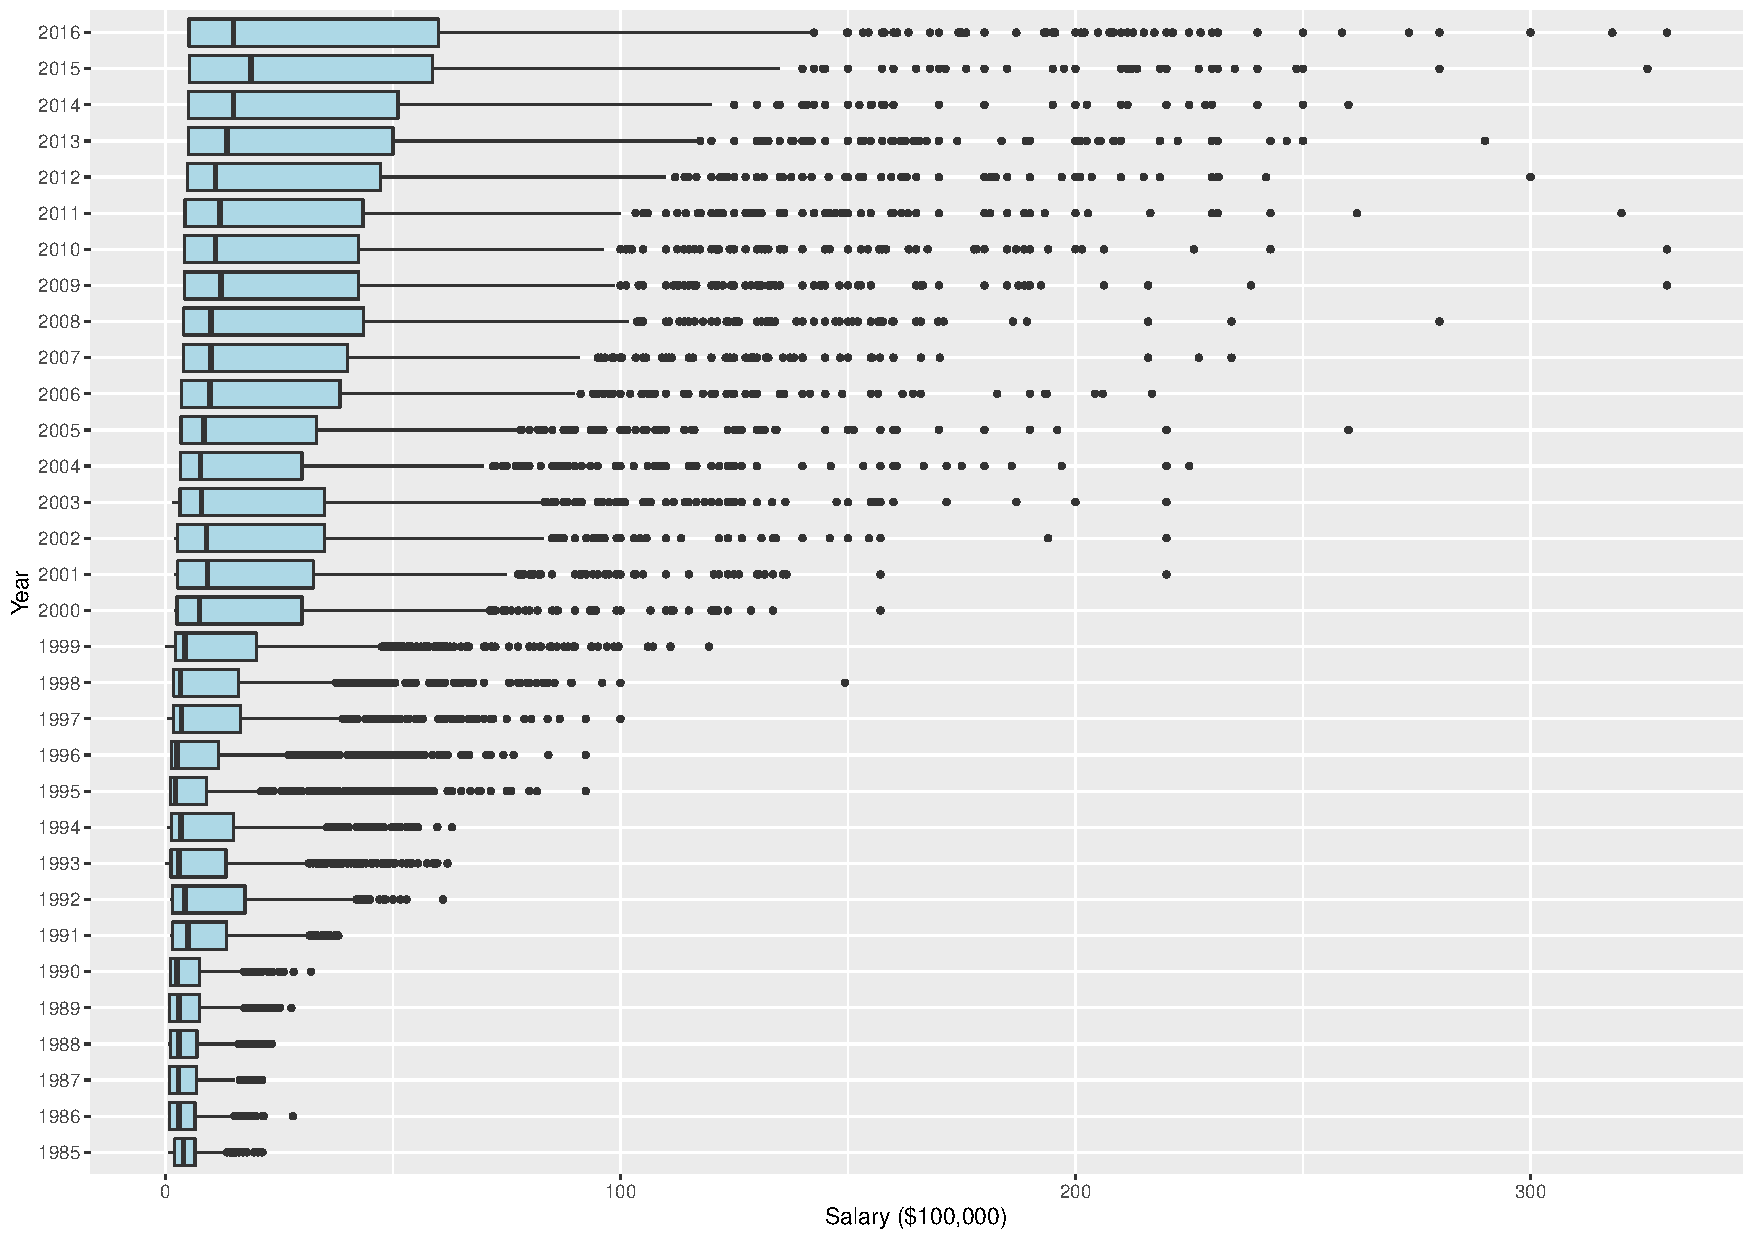
\includegraphics[width=10cm]{photographs/Salaries.pdf}
    \caption{Baseball Salaries over the years}
    \label{fig:Salary}
\end{figure}
We use data from 2010 to predict a players salary in 2011 given how well the player did. Here is the code to isolate the data:
\subsubsection{Training Data}
\begin{lstlisting}[basicstyle=\scriptsize]
batting <- Batting %>%
  filter(yearID == 2010) %>%
  left_join(select(Salaries, playerID, yearID, teamID, salary), 
            by=c("playerID", "yearID", "teamID"))
str(batting)

batting %>%
  filter(! is.na(salary))

names(batting)
salarybatting = subset(batting, select = -c(playerID, teamID, lgID))
salarybatting[is.na(salarybatting)] <- 0
\end{lstlisting}

\subsubsection{Testing Data}
\begin{lstlisting}[basicstyle=\scriptsize]
nextyear <- Batting %>%
  filter(yearID == 2011) %>%
  left_join(select(Salaries, playerID, yearID, teamID, salary), 
            by=c("playerID", "yearID", "teamID"))
str(nextyear)

nextyear %>%
  filter(! is.na(salary))

names(nextyear)
salarynextyear = subset(nextyear, select = -c(playerID, teamID, lgID))
salarynextyear[is.na(salarynextyear)] <- 0
\end{lstlisting}


\section{Train and Test data}
When building models, we have to give prior information to teach the model what it needs to know.
What happens is that we will split the data into a learning class and a prediction class. 
In the learning class, we will further split the data into \textit{training} and \textit{testing} data, normally with around 70\% of the data being for \textit{training}. 
This is usually done automatically, and randomly, by the algorithm for each model.\\
For each algorithm, the training data will be used to teach the model how each factor affects the output and the testing data will be used to verify the results to make sure that the model is within the bounds of error.
\bigskip\\
For this project, I have created \underline{four} datasets from the full Lahman dataset into 

\section{Notation}
Before we proceed, it is necessary to state the notation that will be used in this paper.
\begin{itemize}
    \item $n$ the number of values at each point
    
    \item $M$ the number of groups we form after splitting/partitioning
    
    \item $\{x_{i},y_{i}\}_{i=1}^{n}$ the full dataset
    
    \item $x_{i}$ the input variables
    
    \item $y_{i}$ the dependent variable
    
    \item $\hat{y}_{i}$ the predicted value $y_{i}$

\end{itemize}
From here, we are able to proceed onwards with Decision Trees.


\chapter{AID, CHAID and The Original Decision Trees}
The idea of decision trees is to split up the data into segments (this is called \textit{segmenting}) and then keep breaking them down until we get suitable groups. This can then be summarized up into a tree which can be displayed to see the paths taken.

\section{Basics on Decision Trees}
Trees are basically graphs to show structure and flow.\\
A general idea is to think of a continuous variable $Y$ and some inputs $X_i ,  i = 0,...,n$. Lets say for simplicity, we have for two variables $X_1, X_2$ (thus creating a 2-D plane), we are able to create two separate regions from a partition, which we then model $Y$ on. This partition is on either $X_1$ or $X_2$. \\
Then, we are able to repeat the process for either one or both regions and model $Y$ on the new partitions and continue to do so until we get to a stopping point.
\\
The first question we ask is \underline{how do we know where to split each branch the tree?}

\section{AID}
\textbf{Automatic Interaction Detection (AID)} was first developed in 1963 by Morgan and Sonquist as a social science problem\cite{AID} as an optimization problem to sequentially partition data in an observation matrix into a binary regression tree \cite{ORAID}.
However, since then, it has proven so useful that it has become the basic building block for Decision Tree methods.

\subsection{AID algorithm}
The notation for this algorithm was based on source \cite{EarlyTree}:

\subsubsection{ANOVA}
Using Analysis of Variance (ANOVA), we can calculate the following:
\medskip\\
For a value $y_{im}$, $i \in [1,\dots,n]$, $m \in [1,\dots,M]$.
\begin{description}
    \item[Residual Sum Squares (RSS)] - The sum of the squares of residuals for each group (Also known as Within Sum Squares (WSS))
    \begin{equation}
        RSS = \sum_{m=1}^{M} \sum_{i=1}^{n} (y_{im} - \Bar{y}_{m})^{2}
    \end{equation}
    \item[Total Sum Squares (TSS)] - The sum of squares for all values
    \begin{equation}
        TSS = \sum_{m=1}^{M} \sum_{i=1}^{n} (y_{im} - \Bar{y})^{2}
    \end{equation}
    \item[Between Sum Squares (BSS)] - where BSS = TSS $-$ RSS. Which is equivalent to the sum of squares for regression.
    \item[$\eta^2$] - A coefficient we aim to maximise. This is the ratio: $\frac{BSS}{TSS}$
\end{description}

\subsubsection{Steps for AID algorithm}
The AID algorithm is performed stepwise - it starts with a single cluster and calculates the splits one step at a time until a stopping point is reached. 
\begin{enumerate}
    \item At each step, for each predictor, either of the following occurs \cite{WilkinsonAID}:
    \begin{itemize}
        \item \textbf{Continuous Predictors} - For all $n$ cases, we have $n-1$ ways to split the cluster.
        Calculate the RSS value and select the optimal value.
    
        \item \textbf{Categorical Predictors} - All $2^{k} - 1$ possible splits between $k$ categories are checked.
        Calculate the RSS value and select the optimal value.
    \end{itemize}
    \item After calculating all RSS values we select the point with the          smallest RSS value.

    \item We then consider the \textit{interaction} between predictors as we move down the levels as we no longer consider the same predictors for separate branches of the tree for the next stepwise calculation.
    
    \item Repeat the process until stopping point is reached.
\end{enumerate}

\section{CHAID}
\textbf{CHAID} was developed by Kass in 1980 \cite{CHAID}.
It is essentially an extension of the AID algorithm suited for classification and stands for Chi-square Automatic Interaction Detection.\\
CHAID uses chi-squared statistical significance to test for significance of variables:
\begin{equation}
    \chi^{2} = \sum_{i = 1}^{n} \frac{\sqrt{(y_{i} - E(y_{i}))^2}}{E(y_{i})}
\end{equation}
Where $E(y_{i})$ is the expected value of $y$.

\subsubsection{CHAID Algorithm}
Here we state Kass's CHAID algorithm \cite[pp. 121]{CHAID}.\\
For a given data table with a contingency table, we perform the following algorithm on the table:
\begin{enumerate}
    \item For each predictor, perform cross-tabulation of categories and then do the following:
    \begin{enumerate}
        \item Pair up categories of predictors which are the least significantly different. Merge both if they do not reach the critical value of the $\chi^{2}$ significance test above
        
        \item Repeat this step until all similar pairs have been merged
        
        \item For categories formed from \textbf{at least two} merges, find the most significant binary split and perform a $\chi^{2}$ test to see if this split is significant
        
        \item Repeat until splits are no longer significant
    \end{enumerate}
    
    \item Calculate the significance of each merged predictor and select the highest chi-squared value. If that value turns out to be larger than a criterion value, split the data into subcategories
    
    \item Repeat until all partitions have been analysed
\end{enumerate}
\textbf{Note:} Here, we check the criterion value against a contingency table.
An issue arises when we reduce the table size when merging groups as this means we can no longer use the same contingency table as before.
Kass noted this when formulating the algorithm and proposed using Bonferroni corrections on the splitting criterion which he found to have improved the results. 
We will not go into detail of that but the reader may consult \cite[pp. 122-126]{CHAID} if they would like to look into this.



\section{Downsides of AID/CHAID}
AID and CHAID, while useful, suffers from some issues:
\begin{enumerate}
    \item They are heuristically greedy - The algorithm works in a top-down approach.\\
    Unfortunately, this is a computational constraint and comes up quite often in future methods.
    
    \item Stopping point not defined - The nature of the algorithm means that there is no defined stopping point unless defined by the user when initializing the algorithm. This leads to unnecessarily large trees which require pruning.\\
    This will be solved in CART and will be discussed in the next chapter.
    
    \item Focus not on prediction - The creators of AID/CHAID were more interested in segmenting data than making predictions. Therefore the splits are more associative than a data scientist would prefer.\\
    Nevertheless, we should not ignore AID/CHAID based on this alone and it is still useful, however, not optimal.
\end{enumerate}

\chapter{Modern Decision Trees}
To address flaws in optimizing AID/CHAID, modern methods to form decision trees were invented in the 1980s and are still used today.\\
\textbf{CART} was first introduced by Leo Breiman in his 1984 book Classification and Regression Trees \cite{BreimanDT}.
Since then, it has become one of the most cited methods for machine learning since it is easy to interpret while maintaining its accuracy.\\
An alternative method was developed in 1986 by Ross Quinlan \cite{Quinlan} called \textbf{ID3}, which grew to become \textbf{C4.0, C4.5, C5.0 etc}. The method is very similar to Breiman's and really only differs in terms of the metrics used.




\section{Classification}
To find the best split for Classification Trees, we try to find the split which gives the least errors. This can be defined as a metric to simplify calculations.
We find that there are \textbf{three} major metrics that are used in deciding where to split each branch, of which the first two are the most common.

\begin{enumerate}
    \item \textbf{\textit{Gini Impurity}}: Used by the CART method \cite{BreimanDT}, 
    
    \item \textbf{\textit{Information Gain}}: Used in methods such as C4.5, ID3 \cite{Quinlan}
    
    \item \textbf{\textit{Misclassification Error}}
\end{enumerate}

\subsection{Calculating metrics}
We find that these metrics are based on the idea of Entropy, which itself is part of \textbf{Information Theory}, defined by Claude E. Shannon in 1948 in his landmark paper "A Mathematical Theory of Communication". \footnote{http://cm.bell-labs.com/cm/ms/what/shannonday/shannon1948.pdf} \cite{Shannon}.

\subsubsection{Entropy}
\begin{definition}[Entropy]\cite{Shannon}
The Entropy of a random variable is defined as the information uncertainty in the variable's possible outcomes.
\end{definition}
In fact, Shannon had formulated this into a theorem for entropy which we will now state:
\begin{theorem}[Entropy] [Based on source \cite[Section 6, p. 10]{Shannon}]\\
For a measure $H(p_1,\dots,p_n)$ where $p_1 + \dots + p_n = 1$ with the following conditions:
\begin{enumerate}
    \item $H$ is continuous in $p_i$
    
    \item If all $p_i$'s are equal, then $H$ is monotonic
    
    \item If a choice is broken down into two successive choices, then $H$ becomes the sum of each individual values.\\
    \textbf{For Example}: $H(\frac{1}{2}, \frac{2}{5}, \frac{1}{10}) = H(\frac{1}{2}, \frac{1}{2}) + \frac{1}{2}H(\frac{4}{5}, \frac{1}{5})$
\end{enumerate}
If the above is satisfied, we can define entropy as:
\begin{equation}
    H(T) = I_E (p_1, \dots , p_n) = -\sum_{i=1}^{n} p_i \log_b p_i
\end{equation}
\end{theorem}
In this case we have to derive two forms of entropy:

\begin{enumerate}
    \item Entropy of one attribute (Parent Entropy):
    \begin{equation}
        H(T) = -\sum_{i=1}^{n} p_i \log_2 p_i
    \end{equation}
    This is the full data
    
    \item Entropy of two attributes (Child Entropy):
    \begin{equation}
       H(T \mid a) = -\sum_{i=1}^{n} P(i \mid a) \log_2 P(i \mid a) 
    \end{equation}
    This is the filtered data and the sum of each Child Entropy is equal to the Parent Entropy
\end{enumerate}
We then use the two entropy's to calculate information gain.

\subsubsection{Information Gain}
\begin{definition}[Information Gain]
Information Gain can be defined as the following:
\begin{equation}
    I_G(T,a) = H(T) - H(T \mid a) = -\sum_{i=1}^{n} p_i \log p_i
    + \sum_{i=1}^{n} P(i \mid a) \log_2 P(i \mid a) 
\end{equation}
\end{definition}
Information Gain is used to decide on which feature to split on. We want it so that each split provides the most "information" and is therefore the value with this highest $IG(T,a)$. If $IG(T,a) = 0$, then we have found a leaf node and stop, else repeat the process until we arrive at a leaf node.\\
This is used in ID3 and C4.5 \cite{Quinlan}. We will come back to this later when we progress onto more additive models.

\subsubsection{Gini Impurity}
CART uses a method called \textbf{Gini Impurity} which measures how often we would incorrectly sort a random element from the set. 

\begin{definition}[Gini Impurity]\footnote{https://en.wikipedia.org/wiki/Decision\_tree\_learning}
The Gini Impurity (Also called Gini Index) can be defined as the following:
\begin{equation}
    I_G (p) = I_G (p_1, \dots, p_n) = \sum_{i=1}^{n} p_i(1-p_i) 
\end{equation}
\end{definition} \cite[Metrics]{TreeWiki}

\subsubsection{Misclassification Error}

\begin{definition}[Misclassification Error]
The last measure of node impurity we have is Misclassification Error.
\begin{equation}
    I_G (p) = 1 - \max (p_i, 1 - p_i)
\end{equation}
\end{definition}
Misclassification error is useful when we look at pruning the tree later down the line.




\subsubsection{Whats the difference?}
While the two methods require different calculations, there is no significant difference between Information Gain and Gini Impurity in the results to determine which is more optimal. 
However, when implemented into algorithms, CART, which uses Gini Impurity, while more efficient, can only partition the data into two groups whereas ID3 and C4.5 are able to split into multiple partitions at each point.\\
On the other hand, CART, by the nature of Gini Impurity, provides an efficient stopping algorithm which does not depend on restrictions put on by the user. This makes it the preferred method compared to Quinlan's method.\\
Thus deciding on which to use depends on the end user and their preferences from the results of the algorithm. For now we will proceed with CART.


\subsection{CART Classification Algorithm}
The CART algorithm for classification is very similar to those we have already seen before. \\
For each variable $x_i$, $i \in [i, \dots, n]$ leading to a response $y_i$ where $y$ is a classification, we complete the following:
\begin{enumerate}
    \item For each variable at every point, split the data into two regions $R_1, R_2$ where:
    \begin{enumerate}
        \item $R_1 = x_i \leq s$
        \item $R_2 = x_i > s$
    \end{enumerate}
    
    \item Calculate the Gini Impurity for said split and test it against all other splits
    
    \item Select the value with the highest Impurity as the choice of split
    
    \item Repeat until stopping criterion is met
\end{enumerate}




\section{Regression Trees}
Unlike classification, regression does not have natural groupings to simply work out calculations for where to split. 
Therefore an alternative method for partitioning needs to be found.\\
The method is to minimize the Residual Sum of Squares (RSS), similar to AID but with some differences.\\ 
We have that \cite[Section 3, p. 44-46]{ESL}:

\begin{equation}
  RSS = \sum_{i}^{n}(y_i -\hat{y_i})^2  
\end{equation}

\subsection{CART Regression Calculations}
\emph{Based off ESL \cite[Section 9, p. 307]{ESL}}\\
Suppose we have a space $R$ and we have $M$ partitions, we first partition the space into $M$ regions $R_1, \dots, R_M$.
Our aim is to predict which region the values $x$ fall into and take the average value of the region to make a predictor.\\
To construct the regions, we try to find regions which minimize RSS, where we have $\hat{y}_{R_m}$ as the mean response for each region:
\begin{equation}
    RSS = \sum_{m=1}^{M} \sum_{i \in R_m} (y_i - \hat{y}_{R_m})^2
\end{equation}
To construct this we use the following methods:
\subsubsection{Splitting points using RSS}
We have for each variable $x_i$, $i \in [1, \dots, n]$, leading to a predicted value $y_i$ 
\begin{enumerate}
    \item For each variable at every point, split the data into two regions $R_1, R_2$ where:
    \begin{enumerate}
        \item $R_1 = x_i \leq s$
        \item $R_2 = x_i > s$
    \end{enumerate}
    
    \item Calculate the following for each split:
    \begin{equation}
     \sum_{x_i \in R_1} (y_i - \hat{y}_{R_1})^2  +  \sum_{x_i \in R_2} (y_i - \hat{y}_{R_2})^2
    \end{equation}
    
    \item Select the minimal value in (2) for each variable and compare with all variables selecting the minimal value as the splitting variable.
    
    \item Repeat until stopping criterion is met
\end{enumerate}

We model the response variable to the data with $N$ observations and $n$ inputs, which each have a response, as a constant $c_m$ in each region:
\begin{equation}
    f(x) = \sum_{m=1}^{M} c_m I (x \in R_m)
\end{equation}
Where we can obtain a optimum $\hat{c}_m$ which we find to be the average of $y_i$ for each region $R$.
\begin{equation}
    \hat{c}_m = av(y_i | x_i \in R_m)
\end{equation}

\subsection{Comparisons with AID}
We notice that both Regression CART and AID calculate the RSS values to figure out the residuals if we were to split at a point.
In fact, the algorithm is pretty much the same, although some minor differences can be found. 
The difference is really found in calculating the predicted value of the new child nodes, however, more often than not, this tends to be the same value in both cases.

\section{Pruning}
Often we get trees which are way too big and unnecessarily complicated when simpler trees often do the trick. 
This leads to overfitted trees which provide high bias and low variance and is therefore unsuitable for regular use.\\
Ideally, we would grow a small tree with a minimum split value at certain point.
However, the heuristically greedy nature of the algorithm would hide a very good split behind a seemingly weak split. 
To get around this, the alternative is to grow a very large tree $T_0$ and \textit{prune} them back to obtain a subtree $T$ instead where $T \subset T_0$.
We call this method \textit{Cost-Complexity Pruning} \cite{BreimanDT}.

\subsection{Cost-Complexity Pruning}
The idea of pruning is to minimise the cost-complexity criterion:
\begin{equation}
    C_{\alpha} (T) = R(T) + \alpha \left|T\right|
\end{equation}
Where $R(T)$ is the learning error, $\left|T\right|$ the number of terminal nodes in tree $T$, and $\alpha$ the regularization parameter.\\
$R(T)$ differs depending on the type of tree we are pruning:
\begin{itemize}
    \item For Classification: 
    \[ R(T) = \sum_{i = 1}^{T} (1 - \max (p_i, 1 - p_i)) \times \frac{n(t)}{n} \]
    Where $n(t)$ is the number of $x_i$'s in each $t$ leaf node and $n$ the total number of $x_i$'s
    
    \item For Regression:
    \[ R(T) = \sum_{m=1}^{T} \sum_{i \in R_m} (y_i - \hat{y}_{R_m})^2 \]
\end{itemize}

\subsubsection{Pruning a Subtree}
To prune a subtree, lets look at an individual subtree $T_t$. 
The aim here is to minimise the following:
\[ 
\begin{split}
    C_\alpha(T-T_t) - C_\alpha(T) &= R(T-T_t)+ \alpha|T-T_t| - (R(T)+ \alpha|T|)\\
    &=R(T-T_t)-R(T)+\alpha(|T-T_t|-|T|)\\
    &=R(T)-R(T_t)+R(t)-R(T) + \alpha(|T|-|T_t|+1-|T|)\\
    &=R(t)-R(T_t) + \alpha(1-|T_t|)\\
\end{split} \]
Which results in the following value of $\alpha$
\[ \alpha = \frac{R(t)-R(T_t)}{|T_t| - 1} \]
\textbf{Note:} If $\alpha = 0$, then we return the whole tree unpruned so we aim to look at cases when $\alpha \neq 0$.

\subsubsection{Algorithm}
The Algorithm for pruning is as follows \footnote{mlwiki.org/index.php/Cost-Complexity\_Pruning}:
\begin{enumerate}
    \item Initialization - Let $T^1$ be the tree obtained with $\alpha^1 = 0$ by minimizing $R(T)$
    
    \item Step 1.1 - Select $t \in T^1$ which minimizes
    \[ g_1 (t) = \frac{R(t)-R(T_t^1)}{|T_t^1| - 1} \]
    
    \item Step 1.2 - Let $t_1$ be this node and let $\alpha^2 = g_1 (t_1)$ which results in $T^2 = T^1 - T_{t_1}^1$
    
    \item Repeat - Repeat the process $i$ times until at cost $k$
\end{enumerate}
This results in the following outputs:
\begin{itemize}
    \item a sequence of trees up to the root node: $T^1 \supseteq T^2 \supseteq \dots \supseteq T^k \supseteq \dots \supseteq T^{root}$
    
    \item a sequence of parameters $\alpha^1 \leq \alpha^2 \leq \dots \leq \alpha^k \leq \dots$
\end{itemize}
We now choose $\alpha^k$ which is our optimal value and then obtain the corresponding tree $T^k$ as our result.


\section{Implementation of CART}
There have been multiple implementations of CART over the years. The most famous of these is \textbf{rpart} \cite{rpart}, which is what we have used for this project. 
Here we will use the two sets of data which were put together in the introduction and I will provide a summary of it below.

\subsection{Examples}
\subsubsection{Classification}

\subsubsection{Regression}




\section{Flaws of CART}
CART, while a major improvement over other methods, does have its flaws like all methods do:
\begin{enumerate}
    \item Heuristically greedy - Similar to AID/CHAID, the top-down approach leads to greedy splits where good splits are hidden behind a split which looks strong, but is actually a terrible split as it masks other more appropriate splits.
    
    \item Binary nature of Split - The Gini Impurity metric only works for binary splits (Each parent node can only split in two and not more than that).\\
    Fortunately, other methods such as ID3 and C4.5 using alternative metrics are able to perform better splits in that regard.
    
    \item Complexity of Trees - This is both taxing in terms of computer memory and in terms of size. \\
    Unfortunately, pruning is the only method to achieve a desirable tree without losing any major splits if we were to grow a very small tree instead.
\end{enumerate}



\chapter{Bagging and Random Forest}
Not content with the flaws of CART, Leo Breiman started working on methods to improve on and ended up with two methods which are closely linked and follow on from each other. While many others tried to improve metric selections, they tend to have their own flaws which make them less useful than CART. Breiman figured out that bootstrapping techniques \cite{bootstrap} were the most efficient method, in the 1990s in terms of computer power, while also providing an improvement over CART.
\bigskip\\
The first is \textbf{B}ootstrap \textbf{Agg}regat\textbf{ing} (Bagging) \cite{bagging} \footnote{As an aside, the editor of that paper was Ross Quinlan, the same person who invented ID3, C4.5} which uses bootstrapping techniques to generate many trees to aggregate. Here, all $n$ features are selected as possible splitting nodes for trees and we \textit{aggregate} all trees to build our model.
\medskip\\
The next stage improvement was \textbf{Random Forests} \cite{randomforest}.
Random Forest uses bootstrapping techniques to train multiple weak learners which create a much stronger model when combined together.
Indeed Random Forests only differ from Bagging in the selection of features as Random Forests only select a subset of features and "vote" on the best features when aggregating the final model
\bigskip\\
These technique are called \textbf{Ensemble Learning} and will come up again since they are the most common methods to improving accuracy on decision trees.

\section{Bagging}
Bootstrap Aggregating (Bagging) involves using multiple learning samples from the $\{x_{i}, y_{i}\}_{i=1}^{n}$ dataset, we collectively denoted these as $\mathcal{L}$. 
We denote each bootstrap sample as $\mathcal{L}_k$ where $k \in [1, \dots, B]$.\\
The aim here is to get an aggregated predictor, made up of individual predictors $\varphi_k$ which is better than the individual predictor, which we will denote the final predictor as $\varphi$. 
This is achieved by taking the average of the bootstrap samples.

\[ \varphi = av_{k = 1,\dots,B} (\varphi_k) \]

In theory, this bagged estimator is:
\begin{equation}
    \varphi = \frac{1}{B} \sum_{k=1}^{B} \varphi_k
\end{equation}
Each bootstrap is drawn at random and with replacement and thus it is possible for repeated trees to occur. 
Thus stronger decision points would tend to outweigh weaker trees as they pull the average towards these decisions.
\medskip\\
We will now follow on from Leo Breiman's paper \cite{bagging} for the procedure needed.

\subsection{Classification}
For each individual tree, we use the same method to construct them as we had previously.
The following procedure is followed for all runs:
\begin{enumerate}
    \item A seed is set to allow for replication
    
    \item The full dataset is split \textit{randomly} into a learning set $\mathcal{L}$ and a testing set $\mathcal{T}$
    
    \item A Classification Tree is constructed from the full $\mathcal{L}$ and the test set $\mathcal{T}$ is run to test the misclassification rate
    
    \item 50 bootstrap sample from $\mathcal{L}$ are drawn randomly, and each make a $\phi$ classifier to form $\phi_1, \dots, \phi_{50}$
    
    \item All 50 $\phi$ classifiers are compared with each other and the most common classifier is selected, else, the class with the lowest error relative to the full Classification Tree is selected and this becomes $\varphi_k$
    
    \item Repeat steps 4-5 $k$ times and average the $\varphi_k$ values to obtain $\varphi$
\end{enumerate}


\subsection{Regression}
Similarly, we use an almost identical meta-algorithm to classification but with some minor differences.
The following procedure is followed for all runs:
\begin{enumerate}
    \item A seed is set to allow for replication
    
    \item The full dataset is split \textit{randomly} into a learning set $\mathcal{L}$ and a testing set $\mathcal{T}$
    
    \item A Regression Tree is constructed from the full $\mathcal{L}$ and the test set $\mathcal{T}$ is run to test the misclassification rate
    
    \item 50 bootstrap sample from $\mathcal{L}$ are drawn randomly, and each make a $\phi$ regression to form $\phi_1, \dots, \phi_{50}$
    
    \item Here, the predictor is $\hat{y}_k = av\phi_k$ is used instead of $\varphi$ where we have the squared error $av(y_n - \hat{y}_n)^2$
    
    \item Repeat steps 4-5 $k$ times and average the $\hat{y}_k$ values to obtain $\varphi$
\end{enumerate}

\subsection{Example}

\section{Random Forests}
Random Forests are a natural development from Bagging as they use very similar techniques for growing ensembles. 
In his paper \cite{randomforest}, which will be replicated here, he noted that while both Bagging and Random Forests are similar, Bagging is akin to "\dots darts thrown at random boxes \dots", Random Forests are much more civilized in nature as they are formed by voting "\dots for the most popular class."


\chapter{Boosting}
While Boosting is similar to Random Forests, there are some subtle differences which make them much more accurate and optimal in terms of making predictions.


\section{AdaBoost}

\subsection{AdaBoost and Random Forests}

\section{xgBoost}

\chapter{Optimizing Trees}
While both Random Forests and Boosting are very accurate predictors, they achieve this by sacrificing interpret-ability. 
This makes it harder to show how each decision is made and is the trade-off necessary in order to achieve higher accuracy. We now return to Decision Trees but under a more modern light using ideas from operations research as a basis for the algorithm.



\section{Trees as an Optimization Problem}
Improvements in technology have now allowed us to look at decision trees under a different perspective. 
Historically, the most efficient way to improve accuracy without inducing bias is to look at improving the metrics used for splitting and then when the limits have been pushed, use ensemble techniques to aggregate and minimizing the errors.\\
Dimitris Bertsimas and his PhD student, Jack Dunn proposed reforming decision trees as an optimization problem \cite{oct}. 
This is actually a realisation of Leo Breiman's dream to solve the entire decision tree in one go.
In fact, in CART, Breiman noted the following \cite[p.42]{BreimanDT}:
\bigskip\\
\say{\textit{Finally, another problem frequently mentioned (by others, not by us) is that the tree procedure is only one-step optimal and not overall optimal. ...If one could search all possible partitions ...the two results might be quite different.\\
This issue is analogous to the familiar question in linear regression of how well the stepwise procedures do as compared with ‘best subsets’ procedures. We do not address this problem. At this stage of computer technology, an overall optimal tree growing procedure does not appear feasible for any reasonably sized dataset.}}
\bigskip\\
Thus, really we should now look at the problem as a Mixed-Integer Optimization Problem (MIO).\\
Revisiting CART, we can now look at this as a programming problem called the \textbf{Optimal Tree Problem}.\\
\begin{definition}
    Given a complexity parameter $\alpha$ controlling the tradeoff between accuracy and complexity, a minimum number in each node $N_{min}$ and a dataset $\{x_i, y_i\}_{i=1}^{n}$ we aim to solve the problem $\forall \ l \in leaf(T)$:
    \[ 
    \begin{array}{r@{}r@{}}
        \text{minimize} \quad &{} R(T) + \alpha \left|T\right|\\
        \text{s.t.} \quad &{} N(l) \geq N_{min}
    \end{array} \]
    Where $N(l)$ is the number of points in leaf node $l$ and $R(T)$ is the misclassification error from before.
\end{definition}



\bibliographystyle{apalike}
\bibliography{reference}

\end{document}